% When using TeXShop on the Mac, let it know the root document. The following must be one of the first 20 lines.
% !TEX root = ../design.tex

\chapter{Workflows}

% Abstract. What is the problem we want to solve?
A workflow is a directed graph, where nodes represent processing steps and edges represent data flow. A processing step can only execute when all data from incoming edges is available. It then performs its processing, and the output is eventually provided over the outgoing edges. Workflow is a recursive concept in that a node may contain another (nested) workflow. Special nodes are provided for modeling control flow (loops, branches).

\section{Requirements}

\subsection{Non-functional}

\begin{enumerate}
	\item \label{enum:NFR:W1} Usability: Developing a workflow out of existing modules should be easy and not require programming skills
	\item \label{enum:NFR:W2} Security: Developing/editing workflows must not introduce security risks (like arbitrary code execution)
	\item \label{enum:NFR:W3} Extensibility: Workflows should be expressive enough for anticipated future needs. 
	\item \label{enum:NFR:W4} Scalability: Workflows should allow compact representations that fit into the memory of individual machines. Whenever possible, workflows should facilitate parallel processing.
	\item \label{enum:NFR:W5} Maintainability: Workflows should be modular for easy reuse.
\end{enumerate}

\subsection{Functional}

\begin{itemize}
	\item Multiple in-/out ports per module
	
		Reason: Obvious

	\item Workflows must be specifiable in a simple domain-specific language

		Reason: NFR \ref{enum:NFR:W1}, \ref{enum:NFR:W2}: Only alternative is creating workflows programmatically, a clear violation of the NFRs.

	\item Workflows must have intuitive graphical representations (and eventually facilitate GUI tools)
		
		Reason: NFR \ref{enum:NFR:W1}

	\item Control flow

		Reason: NFR \ref{enum:NFR:W3}, \ref{enum:NFR:W4}: Do not force developers to hide control flow in modules, which the scheduler could then only treat as black boxes.
		\begin{itemize}
			\item Data parallel execution (either due to parallelizable loop or parallel graph) 

				NFR \ref{enum:NFR:W4}
			\item Loops with dynamic exit conditions

				NFR \ref{enum:NFR:W3}. This is needed for any iterative algorithm.
			\item Conditional execution paths

				NFR \ref{enum:NFR:W3}.
		\end{itemize}
	\item Workflows must be embeddable in other workflows, and thus be recursive structures
		
		Reason: NFR \ref{enum:NFR:W5}
\end{itemize}

\section{Workflows and Modules}

A workflow is a directed acyclic graph where nodes represent modules, and edges represent data dependencies between modules. Workflows and modules are recursive concepts in that a module may contain a sub-workflow (i.e., a subgraph). A module defined as a workflow is called \emph{composite module}, a non-composite module is called a \emph{simple module}.

Each module contains a list of ports through which data flows. The computational model for a module is simple: It takes its input through its in-ports, performs processing, and then returns output through its out-ports. When modeled as a graph, each node is hence labeled with a list of input and a list of output ports. Each edge is labeled with a source port (which must be one of the source node's output ports) and a destination port (one of the destination node's input ports).

For composite modules that contain nested modules, additional rules apply that allows linking between the two nesting levels: An in-port of a composite module may also serve as an out-port for connections to the nodes within the composite module's subgraph. Likewise, the out-ports of a composite module may be in-ports for edges from its subgraph's nodes. Edges between different subgraphs are otherwise not allowed. Moreover, an edge may only connect ports that are \emph{type-compatible}, as described in Section~\ref{sec:TypeSystem}.

\begin{example}
Before describing the different modules in detail, it is helpful to look at an example, as shown in Figure~\ref{fig:WorkflowExample}. It shows how logistic regression could be implemented as a CloudKeeper workflow. The informal description is: Take a file with data points, split this files into manageable chunks, then compute matrix $A := X^T D X$ and vector $\vec b := X^T D \vec z$ for each file separately ($X$ is the design matrix corresponding to only that file, and $D$ and $z$ are transformations of $X$ and $\vec \beta$), sum up all $A$'s and $\vec b$'s over all files, compute $\vec \beta := A^{-1} \cdot \vec b$, and iterate until the log-likelihood of $\vec \beta$ has converged.

Note that Figure~\ref{fig:WorkflowExample} is a CloudKeeper-generated GraphViz visualization of a real workflow that should be read as follows: A rectangle represents a module, which is labeled with its instance name (first line) and its module name (second line). Grey rounded boxes represent in-ports of the module, and black rounded boxes represent out-ports. A rounded box with a dotted outline represents a special port like the continue-port of a loop module.
\end{example}

\begin{figure}
	\centering
	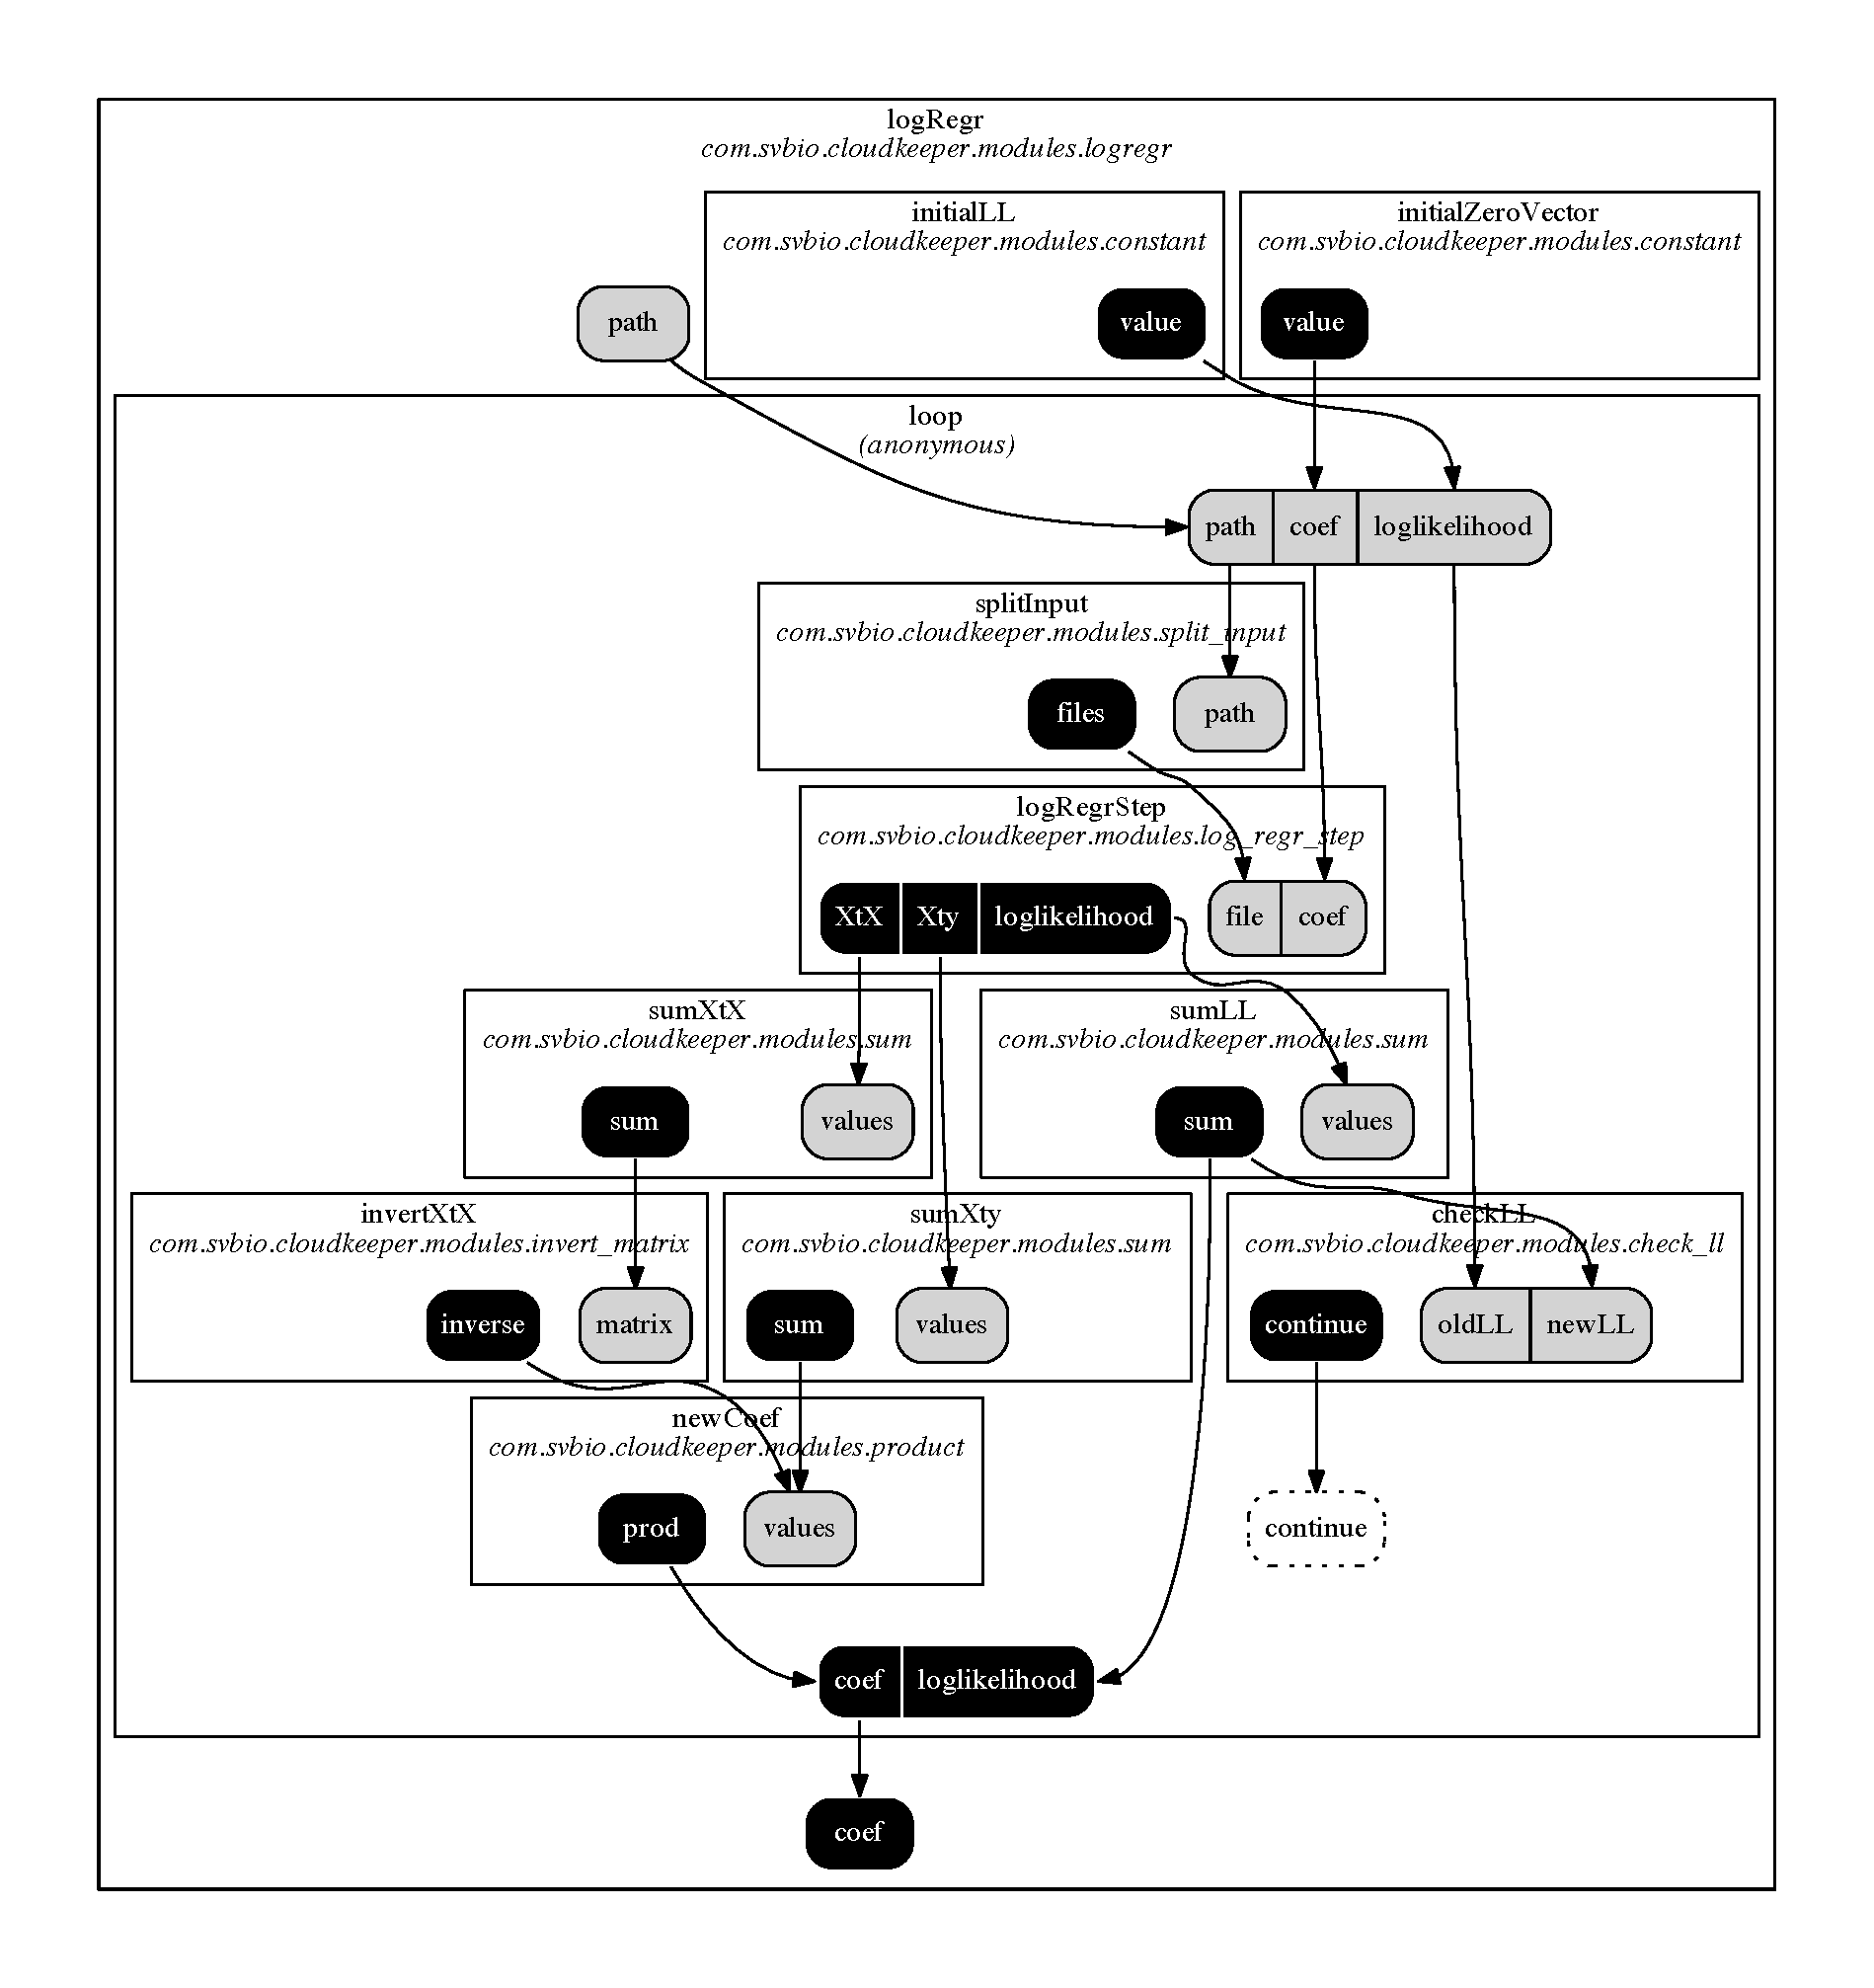
\includegraphics[width=\textwidth]{workflows/workflow-example}
	\caption{Example Workflow: Iteratively Reweighted Least Squares to Perform a Logistic Regression\label{fig:WorkflowExample}}
\end{figure}

\subsection{Module Hierarchy}

Workflows contain module instances that may have one of four different module types:
\begin{enumerate}
	\item Simple Modules
	\item Composite Modules
		\begin{itemize}
			\item Loop Modules
			\item Switch Modules
		\end{itemize}
\end{enumerate}

\begin{figure}
	\centering
	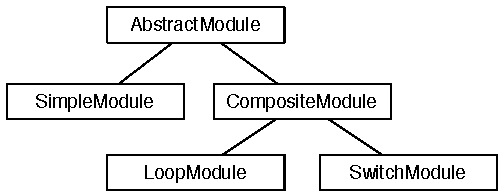
\includegraphics{workflows/module-hierarchy}
	\caption{Module Hierarchy\label{fig:ModuleHierarchy}}
\end{figure}

The hierarchy of modules is also shown in Figure~\ref{fig:ModuleHierarchy}. It is helpful to draw analogies to programming languages:
%
\begin{itemize}
	\item A composite module is a grouping construct for easy reuse of workflows (similar to a block or a function)
	\item A switch module allows the conditional execution of different sub-workflows (similar to a switch/case block)
	\item A loop is the analogue to a repeat-until loop where execution of an iteration (typically) depends on the previous iterations
\end{itemize}

\paragraph{Composite Module}

All composite modules have in- and out-ports just like simple modules. In-ports of a composite module correspond to the formal parameters of a function.

\begin{figure}
	\centering
	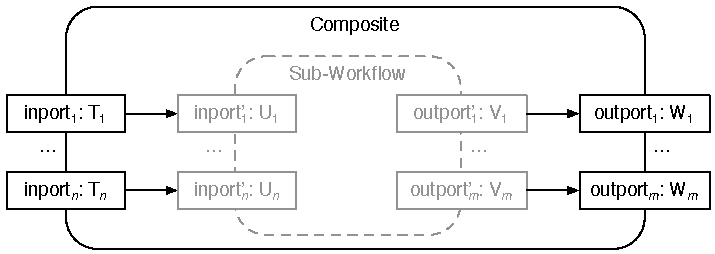
\includegraphics{workflows/composite-module}
	\caption{Composite module. The sub-workflow can be arbitrarily complex.\label{fig:CompositeModule}}
\end{figure}

\paragraph{Switch Modules}

A switch module has a trivial subgraph that consists only of isolated nodes. It has two predefined in-ports: \text{cases} of type \texttt{T[]} and \texttt{value} of type \texttt{T}. On execution, the scheduler will determine the index of \texttt{value} in \texttt{cases}, and then only execute the node in the subgraph with this ID.

\begin{figure}
	\centering
	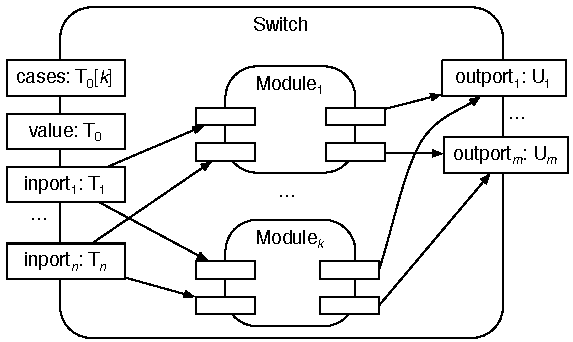
\includegraphics{workflows/switch-module}
	\caption{Switch module. The internal modules may be of arbitrary kind.\label{fig:SwitchModule}}
\end{figure}

\paragraph{Loop Modules}

A loop module has an arbitrary subgraph. Moreover it has a predefined out-port \texttt{continue} of type \texttt{boolean} that determines, after each execution of the sub-workflow, whether the loop module's sub-workflow shoud be executed again. A loop module may have ports that serve both as in\nobreakdash- and out-ports (shown as ``ioports'' in Figure~\ref{fig:LoopModule}). This effectively allows to connect an out-port of the sub-workflow with an in-port of the sub-workflow, in order to pass a value from one iteration to the next.

\begin{figure}
	\centering
	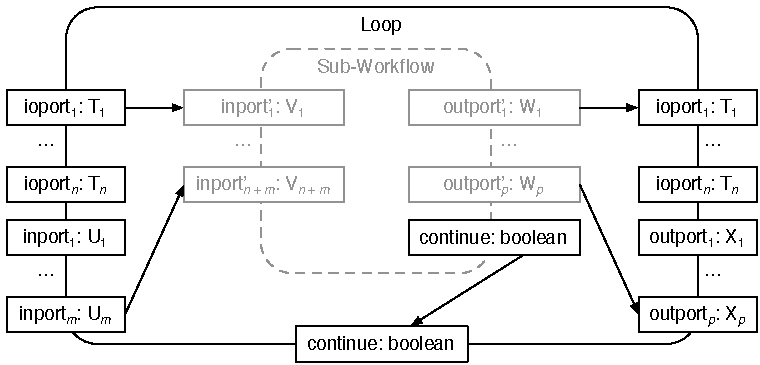
\includegraphics{workflows/loop-module}
	\caption{Loop module. The continue-port is an internal port.\label{fig:LoopModule}}
\end{figure}

\subsection{Data-parallel Module Instances}

Module instances (independent of the module type described before) may be \emph{data-parallel} modules. This property is inferred from the connections a module has in a workflow, as described in the following.

A \emph{split connection} connects an out-port of type \texttt{T[]} to an in-port of type \texttt{U}. Let M denote the module that contains the in-port. A split connection requires that:
%
\begin{itemize}
	\item type \texttt U is type-compatible with type \texttt T,
	\item no other in-port of M has data-parallel connections,
	\item all out-ports of M are connected via a merge connection, i.e., from type \texttt V to type \texttt{W[]}, where \texttt W is type-compatible with type \texttt V.
\end{itemize}
%
A module with split/merge connections is executed using data parallelism, i.e., the module is executed in parallel for each array element of the out-port of the split connection. As part of the merge connection, all out-ports of the module are aggregated into parallel arrays.

\begin{figure}
	\centering
	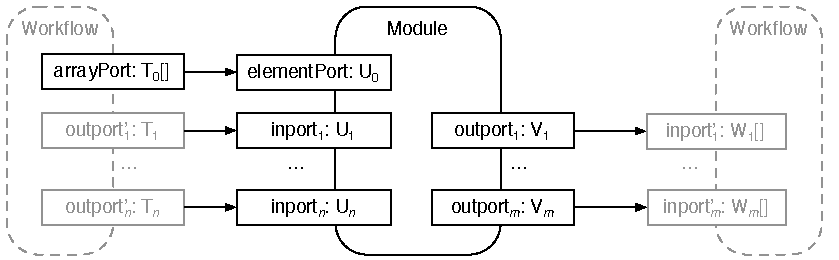
\includegraphics{workflows/data-parallel-module}
	\caption{Data-Parallel module, which may be of arbitrary kind.\label{fig:DataParallelModule}}
\end{figure}

\section{Class Structure} \label{sec:Workflow:ClassStructure}

Workflows are represented by \symlabel{AbstractModule}{sym:AbstractModule} objects. Since the representation contains circular references, these classes are only what is commonly referred to as ``popsicle immutable'': Objects remain mutable until they are explicitly ``frozen''. 
The class structure is shown in Figure~\ref{fig:WorkflowClasses}.

\begin{figure}
\tikzumlset{font=\ttfamily\small}
\centering
\begin{tikzpicture}
	\umlclass[x=10,y=12]{Port}{%
		+ name: String\\
		+ type: Type\\
		+ dimensions: integer
	}{%
		+ freeze()
	}

	\umlclass[x=3,y=12]{AbstractModule}{%
	}{%
		+ freeze()
	}
	
	\umlclass[x=0,y=7]{SimpleModule}{%
	}{%
	}
	\umlinherit[geometry=|-]{SimpleModule}{AbstractModule}
	
	\umlclass[x=6,y=7]{CompositeModule}{%
	}{%
	}
	\umlinherit[geometry=|-, anchor1=70]{CompositeModule}{AbstractModule}

	\umlclass[x=3,y=4]{SwitchModule}{%
	}{%
	}
	\umlinherit{SwitchModule}{CompositeModule}

	\umlclass[x=9,y=4]{LoopModule}{%
	}{%
	}
	\umlinherit{LoopModule}{CompositeModule}
	
	\umluniassoc[geometry=|-|,arg={+ inPorts}, pos=0.9, mult=*, anchor1=90, anchor2=90, arm1=3]{AbstractModule}{Port}
	\umluniaggreg[arg={+ outPorts}, pos=0.3, mult=*, anchor1=-20, anchor2=-152]{AbstractModule}{Port}
	\umluniaggreg[arg={+ inConnections}, mult=*, pos=0.6, angle1=130, angle2=140, loopsize=3cm]{Port}{Port}
	\umluniaggreg[arg={+ outConnections}, mult=*, pos=0.6, angle1=50, angle2=40, loopsize=3cm]{Port}{Port}
	\umluniassoc[arg={+ module}, pos=0.8, mult=1, anchor1=150, anchor2=30]{Port}{AbstractModule}
	\umluniassoc[arg={+ parent}, pos=0.8, mult=0..1, anchor1=-30, anchor2=153]{AbstractModule}{CompositeModule}
	\umluniassoc[geometry=-|, arg={+ modules}, pos=1.8, mult=1..*, anchor1=160, anchor2=-90]{CompositeModule}{AbstractModule}
	\umluniassoc[arg={+ continuePort}, pos=0.9, mult=1]{LoopModule}{Port}
	\umluniassoc[geometry=|-|, arg={+ casePort}, pos=0.6, mult=1, anchor1=-45, anchor2=-65, arm1=-1cm]{SwitchModule}{Port}
	\umluniassoc[geometry=|-|, arg={+ valuePort}, pos=0.8, mult=1, anchor1=-75, anchor2=-45, arm1=-2cm]{SwitchModule}{Port}
\end{tikzpicture}
\caption{Workflow classes.\label{fig:WorkflowClasses}}
\end{figure}
